\chapter{Revisão Bibliográfica}
A pesquisa proposta, assim como os temas abordados nela, é multidisciplinar. As próximas sessões abordarão tópicos necessários para o entendimento do projeto e suas abordagens.

Primeiramente será introduzido a linguística devido ao tema da analise de discurso, essencial para que seja possível analisar como as amostras se expressam em seus textos, além de uma introdução ao processamento de linguagem natural.

Em seguida, será necessário entender sobre Psicologia, dentro dela os tópicos traumas emocionais e modelos de mensuração que serão brevemente abordados devido ao cunho dessa pesquisa. Além disso, será introduzido ao conceito de Psicologia Cognitiva.

Os tópicos já explicados serão utilizados para dar fundamento a Inteligência Artificial. Nessa sessão também seram apresentados os conseitos básicos da área e o conceito de agentes. Em seguida será aprofundado o tema aprendizado de máquina, onde sera explicado conceitos e abordagens utilizadas por essa ramificação da IA.

Por fim, será tratado o tema \textit{data science}, os tópicos relacionados a manipulação de dados, desde a mineração e gestão até a sua representação e organização.

\section{Linguística}
A gramática é composta por: um conjunto finito de letras que formam o chamado alfabeto e um conjunto de regras e normas. Utilizando das regras e do finito número de palavras formadas a partir das letras, é possível se expressar através de uma sentença. O estado representado por essa sentença pode variar de acordo com a regra aplicada. É impossível cobrir todos os estados com uma única regra pelo motivo de existirem números infinitos de sentenças a serem formadas \cite[13-25]{chomsky2002syntactic}. Essa capacidade de obter descrições de forma simplificada através da linguagem é a primeira área cognitiva do ser humano \cite[131]{putnam1975mind}.

No dia-a-dia, existem multiplos fatores que ajudam a entender o sentido de uma frase, porem, em uma máquina os mesmos fatores muitas vezes não se aplicam. Nessa sessão o enfoque é em introduzir alguns estudos fomentados pela linguística. Na inteligência artificial, o ato de juntar símbolos (padrões físicos) em expressões (estruturas) utilizando um conjunto de regras (processos), é considerado um sistema de símbolos físicos. Acredita-se que um sistema desse nesse formato possui os meios necessários e suficientes para realizar ações inteligentes de forma geral \cite[116]{newell1976ComputerSA}. Entretanto, o que foi escrito é diferente do que é compreendido, vide duplo sentidos, logo o contexto é necessário.

% sections
\subsection{Analise de Discurso}
No decorrer de um texto (que é algo concreto), pode-se caracterizar diversos níveis de geração de sentido.
A primeira formulação de sentido vem do discernimento de termos dentro de um contexto, esse nível é chamado de fundamental. Após distinguir esse primeiro sentido ele é aplicado pelo autor através de um sujeito fazendo com que a prosa tome uma direção, esse nível é chamado narrativo. Por fim, existe o nível discursivo, relacionado as escolhas de tempo, espaço, pessoa e figura durante a narrativa dos fundamentos, dando a essa narrativa um ponto de vista. Logo, o termo discurso é dado como um suporte abstrato por trás do texto, afim da concretização da sua ideia central \cite[13-17]{gregolin1995ad}.

A analise de discurso é, de forma sucinta, uma analise do que foi dito, de como foi dito e qual o sentido do que foi dito. As primeiras manifestações do assunto foram no século XX com autores russos que, além de isolar e definir elementos de uma linguagem poética queriam definir determinantes por trás do perfil artístico do escritor. O tempo fez com que a analise de discurso se desenvolvese e ramificasse em várias vertentes, uma delas a francesa, que apoia a possibilidade de automatizar essa analise por meio da informática. A área continua sendo um campo complexo e de contínuo estudo por trás das definições e metodologias para abordar e sustentar as novas unidades de analise. \cite[22]{souza2006ad}.

Os discursos se diferem de pessoa para pessoa devido ao nível discursivo, a necessidade de expressar um determinado sentido leva o autor a se colocar em um ponto de vista durante sua narrativa. Do contexto da pesquisa, entender o discurso do usuário para mapear o motivo do seu estado mental é um fator de total relevância para entender o estado dele. A pesquisa realizada por Modesto Leite \cite[134]{modesto2005adepre}, mostra em seus resultados que os discursos apresentados pelos pacientes fundamentavam o motivo psicológico do por que os mesmo teriam o transtorno. 

Partindo dos principio apresentados sobre um discurso, por mais que as palavras sejam localizadas, o ponto chave da discussão está em como um computador seria capaz de inferir o sentido da frase. Existem áreas, seguindo os campos multidiciplinares que envolvem linguitica e computação, responsáveis por garantir que o processamento dos textos gerará os resultados esperados.

\subsection{Processamento de Linguagem Natural}
Se entender palavras não significa entender o contexto, logo, se familiarizar com o ambiente e o momento afim de idealizar o que está sendo transmitido é algo necessário. Essa conexão entre elementos é tratada no estudo do \textit{connectivism}\footnote{Integração dos princípios de rede, caos, complexidade e teorias de auto-organização. Seu objetivo é entender decisões baseado nas mudanças de componentes fundamentais \cite{siemens2014connectivism}.}. De acordo com a linha de pensamento, estabelecida pelo estudo, os neurônios seriam os agentes cognitivos responsáveis por planejar, construir e representar essas informações que o cérebro humano recebe. Criar soluções para problemas pontuais que envolvam a língua que é utilizado no dia-a-dia se uma pessoa, essa é a definição por trás do Processamento de Linguagem Natural (PLN). Fornecer dados linguísticos que a maquina não é capaz de inferir, ou que seja necessário uma ajuda para seu melhor desempenho, é o ponto principal dessa área \cite{brandura1996, maria2015npl}.

Já que o PLN será inicialmente utilizado para análise de palavras-chaves e padrões, é necessário vislumbrar que será necessário um conjunto de regras a fim de melhorar uma determinada métrica durante o processo de aprendizagem. Para que isso seja possível, um conhecimento dentro da área de psicologia se torna altamente relevante.


\section{Psicologia}

A psicologia é, descrita como, a ciência da vida mental, capaz de analisando os desejos, sentimentos, razões, sentimentos, decisões entre outras faculdades mentais entender o posicionamento e o estado emocional do ser. Entender o nosso estado e como isso impacta em a vida é o grande desafio da área \cite[4-8]{william1890principles}.

Nossa pesquisa utiliza da psicologia em dois pontos distintos, porem, interligados. A primeira delas é o envolvimento da psicologia com a depressão, em segundo a participação da área da psicologia cognitiva na evolução da Inteligencia Artificial. Ambos os pontos se interligam ao se questionar o motivos de alguem ter depressão, ou o quão plausivel é o mapeamento disso através de técnicas desenvolvidas dentro da área nos ultimos anos.

% sections
\subsection{Depressão}
Desanimo, perca de interesse, inibição e bloqueio de sentimentos são alguns sintomas exibidos por pessoas melancólicas \cite[276]{freud}. A \textbf{melancolia} seria uma condição maléfica de enfraquecimento da sáude mental de um ser. Partindo do principio de Fairbain onde o ser humano busca por gratificação, a não gratificação poderia ser o motivo de um estado melancólico.

A \textbf{depressão} é uma forma atenuada de melancolia \cite{roudinesco2000}. Classificada como \textbf{transtorno de humor}, diferente de outras variações mais regulares de humor, pode causar grandes danos a vida cotidiana uma vez que, por definição, altera a percepção de si mesmo maximizando o peso dos seus problemas diante de sua própria pespectiva. Por tais motivos, a melancolia e a depressão compartilham de sintomas similares, entretando, a dinamica de suas origens, relações e concepções podem criar diversas perspectivas o que leva ao ponto de como se pode medir algo tão abstrado. \cite{}

\subsection{Ansiedade}

\subsection{Escala Depressão, Ansiedade e Stress}
Adotando um modelo dividido em 3 sub-escalas a \textbf{Escala de Depressão, Ansiedade e Stress} ou \textbf{EADS} foi proposta na premissa de uma maior assertividade na analise das dimensões afetivas negativas, uma vez que existiam outras pesquisas com proposta similar como o \textit{ Beck Anxiety Inventory} (BAI) e \textit{Beck Depression Inventory} (BDI). As diferenças entre essas escalas são: sua execução, o fator de correlação das sub-escalas propostas pelo EADS e o inventário de Stress introduzido durante o estudo (como mencionado na sessão anterior).  

A EADS completa é composta de 42 itens, por fins de facilitar a geração de dados iremos usar o modelo de 21 itens, que são divididos igualmente entre as escalas e mesmo que um deles pertença a uma escala ele pode ter correlação com alguma outra. Esses itens são afirmações que podem ser respondidas por números de 1 a 4 que representam desde "não se aplica a mim" até "se aplicou a mim na maior parte das vezes" e no final serão somados a fim de gerar um resultado para a sub-escala, os maiores valores representam as dimensões mais negativas \cite{lovibond1995structure, ribeiro2004contribuiccao}.

Diferente da proposta de auto avaliação ou avaliação mediada\footnote{Nesses casos os usuários são responsáveis por responder as perguntas por si mesmos ou por meio de um mediador que ira preencher o formulário.}, como é proposta pela EADS,  uma das premissas da pesquisa é inferir os resultados das escalas utilizando textos cotidianos de uma amostra em rede social. Isso nos leva a entender os conceitos cognitivos por trás da psicologia que levaram os autores a propor suas escalas e pesquisas.



\subsection{Psicologia Cognitiva}
Dentro da Psicologia existe um ramo cujo o objetivo é entender a capacidade animal de pensar, memorizar, perceber e no caso humano utilizar um dialeto (linguagem), essa área de estudo ficou conhecida como psicologia cognitiva.

O ato de entender os procedimentos cognitivos adotados pelo ser humano se tornou mais relevante após a proposta da criação de uma inteligência artificial. O questionamento de como uma decisão poderia gerar, afetar ou cancelar uma cadeia de eventos, seja ela durante um pensamento ou uma ação, partindo da capacidade humana de realizar múltiplas tarefas, algumas delas complexas como interpretar linguagens com tantas divergências, fez com que em 1958\cite[4-7]{broadbent1958perception} surgisse o primeiro modelo psicológico que propunha um fluxo similar ao processamento de informações de um computador.

As técnicas experimentais, como os modelos psicológicos, impactaram toda a área interdisciplinar das ciencias cognitivas. Novas abordagens como a junção de modelos criados em computação para IA e técnicas experimentais da psicologia foram criadas a fim do entendimento da mente humana. Durante a criação do \textit{General Problem Solver}, por exemplo, Newell e Simon propuseram não só a implementação de algoritmos descritos por antigos estudiosos afim de resolver um série de problemas, mas também, entender como a maquina estava realizando isso, assim, seria possível uma comparação com a mente humana \cite{newell1961gps, russell2003artificial}.

Nessa pesquisa, a psicologia cognitiva terá um grande impacto em entender como as amostras que contem ou não sintomas causados pelas dimensões afetivas negativas se comportam e pensam. Esse entendimento é essencial para o mapeamento dos atributos que serão processados pela IA afim de gerar os modelos para predição em dados ainda não analisados. Além disso, a psicologia cognitiva faz parte de todo o processo qualitativo de criação devido a ser um dos vários campos que compões a multidisciplinaridade dentro da IA.

\section{Inteligencia Artificial}

Inteligência é, por definição, uma coleção sistemática de habilidades e funções com objetivo de processar diferentes tipos de informações de diversas maneiras \cite[49]{guilford1982cognitive}. Simular essa "coleção sistemática de habilidades e funções", tais como reconhecer formatos, tragetórias, sinais, deduzir proposições entre outras, afim de criar entidades inteligentes é o foco da inteligencia artificial \cite[1]{russell2003artificial}. Desde que a inteligencia artificial passou a ser um campo de estudo a quantidade de abordagens apresentadas por diversos pesquisadores afim de construir uma máquina inteligente apenas aumentou. Esses métodos se auto-contribuiram até levar a IA para seu estado atual. \cite[2]{russell2003artificial}.
\section{Aprendizado de Maquina}
Se maquinas pensam ou não, o enfoque da IA é executar diretamente um processo que um ser humano aprendeu ao longo dos anos, e não, algo que implicitamente nasceu com ele. Logo, o fluxo mais sistemático para conseguir que uma maquina abstrai-se formalmente um conhecimento seria mapear um estado inicial, aplicar dados para sua aprendizagem e submete-la a outras experiências afim de reafirmar esses conhecimentos. Essa abordagem foi proposta por Turing em 1950, entretanto, o campo de pesquisa conhecido como \textit{\textbf{machine learning}} ou \textbf{aprendizado de maquina} surgiu apenas em 1959 quando o termo nasceu ao ser aplicado em um estudo de redes neurais. Portanto, pode-se brevemente descrever o aprendizado de máquina como métodos computacionais designados a utilizarem de algoritmos precisos de predição juntamente a uma base de conhecimento para aumentar a sua assertividade\cite[1]{turing1950, samuel1959some, mohri2012foundations}.

Nessa sessão será dado um enfoque maior em \textit{machine learning}, primeiramente será introduzido alguns conceitos que serão utilizados a partir dessa sessão. Com os conceitos passados, sera apresentado, de maneira lacônica, conceitos de utilização dos dados e conceitos dentro do aprendizado de maquina, juntamente com sua aplicação por algumas abordagens. Por fim, será sugerido algumas ferramentas utilizadas para implementação do \textit{machine learning} e um breve enfoque em como guiaremos esse campo dentro de nossa pesquisa.

\subsection{Conceitos do Aprendizado de Máquina}
Previamente foi dito que, seriam necessários dados de treino, esse dado bruto, como já dito também, contem várias propriedades que podem ser ou não processadas afim de gerar informações, esse dado é conhecido com dados de treinamento e um dado que contém as informações processadas necessárias, inserida por algoritimos ou por fatores externos, é chamado de dado rotulado ou anotado.

As propriedades podem ser utilizadas para classificar um determinado dado, isso as concede o nome de atributo. Também conhecido com \textit{feature} é considerada como um dos fatores mais relevantes para o aprendizado da maquina. O termo conhecido como \textit{feature engineering} ou, em tradução literal, engenharia de atributos, diferente do processo de aprendizagem em si, são baseados diretamente a suas entidades e em como escolher e pré-processar seus atributos chaves afim de otimizar o aprendizado \cite{domingos2012few}.

Esses atributos, dentre outras propriedades, estão em uma massa de dados. Por sua vez serão utilizadas como dado de entrada para um agente. Esse agente tambem pode ser representado, por fins explicativos, como uma simples função \textit{f(x) = y}, o objetivo é treinar o agente para que ele seja capaz de generalizar. Ou seja, capaz de predizer o melhor valor para \textit{y} a partir da entrada \textit{x}. Quando o resultado final depende totalmente do dado de entrada, ou seja, não existem muitas variações que levem a saída a grandes divergências, dizemos que o problema generaliza bem.

Essa função gerada que sucintamente traduz os padrões encontrados entre os dados, gera o que conhecemos como modelo. Muitos deles são utilizados para classificar o dado dentro de um grupo de possibilidades, esse tipo de modelo é descrito como classificador.

Os problemas a serem processados pelos classificadores ou outros modelos possuem um conjunto de  hipóteses. Quando é concebida uma preferencia a uma dessas hipóteses com a premissa de induzir o modelo a tomar uma decisão chamamos esse ato de tendência.

Uma quantidade extensa de hipóteses e dados de entrada não significam uma maquina mais assertiva, quando um agente é treinado para executar mais do que o necessário, um fenômeno peculiar chamado de \textit{overfitting} ou sobre-ajustes acontece, esse evento faz com que a maquina seja capaz de tomar decisões assertivas apenas para um conjunto de dados a qual foi submetida e não consegue predizer novas entradas.

As descrições dadas por Russel \cite[693]{russell2003artificial} ainda se aplicam a conceitos mais complexos que não cabem a essa pesquisa explicitamente. O jeito que é utilizado os dados ou os atributos previamente ditos, podem resultar em diversos tipos de abordagens diferentes.

\section{Ciência por tras dos dados}
Como um ser humano, os dados têm seu ciclo de vida, esse ciclo pode alterar-se dependendo de sua finalidade dentro da aplicação. O nosso tema e nosso objetivo é coberto por uma matéria, já antiga, nomeada \textbf{KDD} ou \textbf{\textit{Knowledge Discovery in Database}}, embaixo dela existem varias subclasses como mineração de dados, analise de dados, probabilidade e até mesmo IA. A KDD se justifica pela sua metodologia de manipulação de dados afim de extrair o conhecimento almejado de um base. Se observar o fluxo descrito na \ref{fig:kdd}, pode-se notar que uma cadeia de eventos como: seleção, pré-processamento, mutação, mineração e interpretação. Esses eventos geram novos estados para o dado, e os moldam focando o objetivo de retirar o conhecimento pela interpretação no final do processo.

\begin{figure}[H]
    \centering
    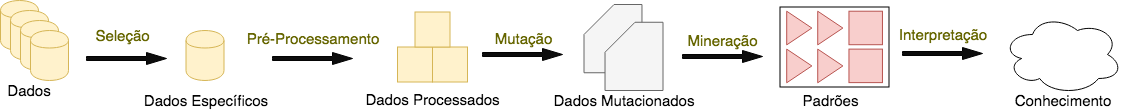
\includegraphics[width=.8\textwidth]{imagens/kdd.png}
    \caption{Representação da metodologia defendida pela KDD. Fonte: o autor.}
    \label{fig:kdd}
\end{figure}

Com o passar do tempo, vários novas abordagens surgiram para tratar dados, e essa massa de pesquisas e definições deu-se por bagunçar um pouco a nomenclaturas e definições que estão atrelados a \textbf{ciência por traz dos dados}. Para evitar confusões as definições apresentadas nessa sessão serão sucintas e tem como objetivo futuros tópicos e discussões apresentados durante os resultados dessa pesquisa. Devido a grande divergência, ocorrido pela disseminação rápida e conturbada de algumas termologias, sobre os temas abordados, serão seguidas as seguintes referencias \cite{laender2002brief, fayyad1996kdd, hand2007principles}.

\subsection{Extração de Dados}
A extração, é o ato de obter dados em massa de fontes externas, como \textit{websites} e \textit{apis}\footnote{A sigla API vem de \textit{Application Programming Interface} e é um interface que permite outras aplicações utilizarem de seus recursos e funcionalidades. Dentro do universo \textit{web}, o termo API é utilizado para descrever um conjunto de rotas que podem ser utilizados para acessar recursos de um aplicação online.}. Esse passo ocorre antes do passo descrito pela KDD como seleção. Conhecido pelo termo inglês \textit{data extraction}, tem sua relevância ao ser a primeira etapa para construir uma base de conhecimento.


\subsection{Seleção de Dados}
O ato de selecionar os dados com enfoque no conhecimento que você deseja obter deles afim de gerar um conjunto de dados especifico é também conhecido como \textit{\textbf{data collection}}, durante o processo do KDD é o primeiro passo responsável por gerar um amostra mais focada no problema.

\subsection{Mineração de Dados}
Nessa subseção propõe-se que seja dissertado sobre os processos do KDD a partir da seleção até a interpretação. Vale ressaltar que para obter conhecimento não é necessário uma IA, sistemas de tomada de decisão trabalham com probabilidade matemática sob dados exatos, o que em muitos casos, já seria o suficiente para obter a informação do dado. Entretanto, o foco da pesquisa se baseia na implementação de um sistema inteligente e isso inclina essa explicação para o fato de: o aprendizado de máquina é uma das possíveis formas de se minerar um dado.

A mineração de dados ou popularmente conhecida como \textit{data mining}, baseia-se em retirar os valores mais relevantes e valiosos para se inferir um conhecimento. Os demais passos como pré-processamento e mutação se assemelham a alguns processos citados anteriormente como a redução dimensional ou ainda a engenharia de atributos.


\subsection{Analise de Dados}
E finalmente, a analise. O passo descrito como interpretação no KDD se refere a entender os dados de saída vindos da mineração afim de afirmar ou descarta hipóteses, com isso é possível refinar o processo e explorar novas possibilidades. Uma das palavras que hoje se tornaram popular dentro dá área é o \textit{data storytelling}, ou, o ato do dado de contar uma história. Abordar a hipótese de maneira empírica e demonstrar a veracidade dela discutindo abordagem e algoritmos gerados é um dos objetivos dessa área.





